\newpage

\appendix
\setcounter{figure}{0}
\renewcommand{\thefigure}{S\arabic{figure}}
\setcounter{table}{0}
\renewcommand{\thetable}{S\arabic{table}}
\onecolumn


\section{Impact Statement}
\label{sec:impact}
In this paper, we focus on the abstract problem of visual exploration -- how to interact with the environment to locate the objects of interest. To evaluate this ability in VLMs, we propose a benchmark designed around flying a UAV to find objects in urban and natural environments. This is relevant to real-world applications with positive societal impact, such as search-and-rescue missions, forest fire detection, or personal assistance. However, autonomous UAVs also pose risks as they can be misused by bad agents for surveillance or military operations. We implore users to use their best judgment for the use of the benchmark. Our benchmark is not designed for surveillance or military applications. We urge other researchers to ensure that their benchmarks (including FlySearch derivatives) and models are not directly or indirectly optimized for malicious objectives. We encourage researchers to evaluate their systems for potential biases or unintended behaviors that could lead to misuse. Finally, we would like to highlight the importance of regulatory oversight and the need for clear ethical guidelines in the deployment of autonomous UAVs.

\section{Funding Transparency Statement}
\textbf{Funding.} All financial activities supporting the submitted work are listed in the \nameref{sec:acknowledgments} section of the main paper. 

\textbf{Competing Interests.} At the time of the publication, Maciej Wołczyk is working at Google. However, he did the majority of the work on this paper while at IDEAS NCBR and has not been involved in benchmarking Google models. The authors declare that they have no competing interests and no financial relationships with any entity that could be perceived as influencing the content of this work.


\section{Benchmark specification}

In this section we present the parameters of benchmark scenario generation and evaluation details.
\subsection{Scenario parameters}

% Please add the following required packages to your document preamble:
% \usepackage{multirow}
\begin{table*}[th]
\centering

\caption{\textbf{Parameters in scenario generation:} In this table, we present value ranges for variables that have an impact on the search trajectory. We sample from them uniformly at random while creating a scenario. \anomalychallenge{} has identical value ranges to \challenge{}, except for the searched object type and searched object asset. Furthermore, in \challenge{} and \anomalychallenge{} there will be a clear line of sight from the starting position of the agent to the object. In \hardchallenge{}, we relax this condition and only validate that the object is not under an obstacle (e.g. is not hidden under a bridge, but can be behind a building). Lastly, objects can be placed anywhere in the forest environment and in one of \(31852\) semantically correct locations in the city environment.}
\begin{scriptsize}
\begin{tabular}{lccc}
\toprule
\multirow{3}{*}{Parameter} & \multicolumn{2}{c}{\challenge{}} & \hardchallenge{} \\ 
\cmidrule(lr){2-3} \cmidrule(lr){4-4} \\ 
 & Value range (Forest) & Value range (City) & Value range (City) \\ \midrule
Seed & \( \mathbb{N} \cap [0, 1000000000]\) & \( \mathbb{N} \cap [0, 1000000000]\) & \( \mathbb{N} \cap [0, 1000000000]\) \\ \midrule
Agent's starting height (\(h\)) [m] & \(\mathbb{N} \cap [30, 100]\) & \(\mathbb{N} \cap [30, 100]\) & \(\mathbb{N} \cap [100, 125]\) \\
Agent's starting position offset [m] & \([-0.5h, 0.5h] \) & \([-0.5h, 0.5h] \) & \([-0.95h, 0.95h] \) \\ \midrule
Searched object type & \{campsite, trash, person, fire, building\} & \multicolumn{2}{c}{\{construction works, crowd, trash, fire, car\}}  \\ 
Searched object coordinates & Anywhere on the map & \multicolumn{2}{c}{38152 possible placements}  \\ 
Searched object asset & Dependent on the object type & \multicolumn{2}{c}{Dependent on the object type}  \\ \midrule 
Sun elevation angle & \([10, 90]\degree\) over horizon & $45\degree$ over horizon & \([10, 90]\degree\) over horizon \\ 
Sun azimuth angle & \([0, 360]\degree\) & $110\degree$ & \([0, 360]\degree\) \\ 
Tree density & \([0.0, 0.3]\) & N/A & N/A \\ 
Rock density & \([0.0, 0.1]\) & N/A & N/A \\ 
\midrule 

Object visibility & \multicolumn{2}{c}{Visible from agent's starting position} & Not under an obstacle \\ 

\bottomrule
\end{tabular}
\end{scriptsize}

\label{knobs}

\end{table*}

\label{sec:genparams}

We present all variables that can be used to generate a new scenario in Table \ref{knobs}, such as whether the searched object should be visible from the UAV's initial location. In Table \ref{scenario-params}, we describe additional parameters that do not impact the scenario generation, but govern details of evaluation -- such as: 
\begin{itemize}
    \item Search area bounds -- a rectangle centered on agent's initial position, describing bounds inside of which agent can move. Note that this only serves as a limitation on agent's movement and does not impact the scenario generation process,
    \item Maximum altitude -- if an agent's action would bring it above that threshold, it is considered invalid and the agent is asked to issue a new instruction,
    \item Whether agent can move beyond its \textit{current} view -- in \challenge{} and \anomalychallenge{} the agent is prevented from leaving visible area, discouraging hallucination,
    \item Number of available actions,
    \item Number of possible \textit{consecutive} retries if agent's action is considered invalid and needs to be redone,
    \item Whether the agent should also receive an image showcasing how the target object should look like from above.
\end{itemize}
\begin{table*}[th]
\centering
\caption{\textbf{Additional parameters:} In this table, we present configurations used during evaluations in \challenge{}, \anomalychallenge{} and \hardchallenge{}. Number of possible retries in case of invalid action was introduced to prevent LLMs from "hanging" by constantly performing invalid actions. As such, this limit was not present while evaluating human baselines. Similarly, we allow humans to fly out of their current view even in \challenge{}. We note that \challenge{} and \anomalychallenge{} use the exact same configuration, while more search-oriented \hardchallenge{} uses a slightly different one. In this table, \(h\) denotes starting height of the UAV. }
\begin{scriptsize}
\begin{tabular}{lcc}
\toprule

Parameter & \challenge{} / \anomalychallenge{} &\hardchallenge{} \\
\midrule 

Search area bounds [m] & \(400 \times 400\) & \(2h \times 2h\) \\ 
Maximum altitude [m] & \(120\) & \(300\) \\ 
Agent can move beyond its current view & No (Yes for humans) & Yes \\ 
Number of available actions & 10 & 20 \\
Number of possible retries if action is invalid & 5 (\(\infty\) for humans) & 5 (\(\infty\) for humans) \\
Object type specification modality & Text & Text + Image \\ 

\bottomrule
\end{tabular}
\end{scriptsize}

\label{scenario-params}

\end{table*}


\subsection{Target details}
The targets in the City environment are as follows:
\begin{itemize}
    \item Road construction works -- a construction zone at the side of a road,
    \item Crowd -- a group of over 30 randomly generated people standing close together,
    \item Large trash pile -- a random pile of trash (bags, car tires, barrels, metal sheets, etc.),
    \item Fire -- a burning car or pile of trash with fire and smoke,
    \item Car -- a randomized car or truck with a specific color (we provide the agent with the color and type).
\end{itemize}
While in the Forest the goal is to find:
\begin{itemize}
    \item Campsite -- a randomly generated set of camping equipment, including at least one tent,
    \item Trash pile -- a pile of car tires, barrels, metal scrap, and other waste (different than in the forest environment),
    \item Person -- a human laying flat on the ground, representing an injured hiker,
    \item Forest fire -- a burning forest area, emitting a large cloud of smoke,
    \item Building -- an abandoned building in various styles.
\end{itemize}


\section{Human baselines}
\label{app:human_baseline}
In order to evaluate human performance on \ours{} we provide a web-based interface for human testers. The interface is designed to be consistent with VLM evaluation procedure, while allowing for efficient human interaction. Therefore, instead of using XML formatted text for communication, the interface uses standard HTML forms and buttons. In Fig.~\ref{fig:web-start} the welcome screen is presented. The user is shown the model prompt (with XML formatting instructions omitted) and can select the between \challenge{} and \hardchallenge{}. In Fig.~\ref{fig:web-fs1} and Fig.~\ref{fig:web-fs2} the communication screens for \challenge{} and \hardchallenge{} respectively are shown. On each step the evaluator has to either fill in X, Y, Z action coordinates and press the \texttt{MOVE} button, or if they believe they have fulfilled the task criterion they have to press the \texttt{FOUND} button. Finally, after clicking \texttt{FOUND} or exhausting possible moves the user is notified if they have succeeded or failed the scenario. During the entire evaluation, users can report any issues with a built-in bug report form. 

Source code of the interface and associated back-end server is included in \ours{} codebase. The study was conducted with participation of human manual software testers (employees). The study did not pose any risks to participants. No Personally Identifiable Information was gathered in the process. The study was conducted according to institutional regulations on data gathering and processing and was subject to internal approval process.



\begin{figure*}[ht]
    \centering
    \fbox{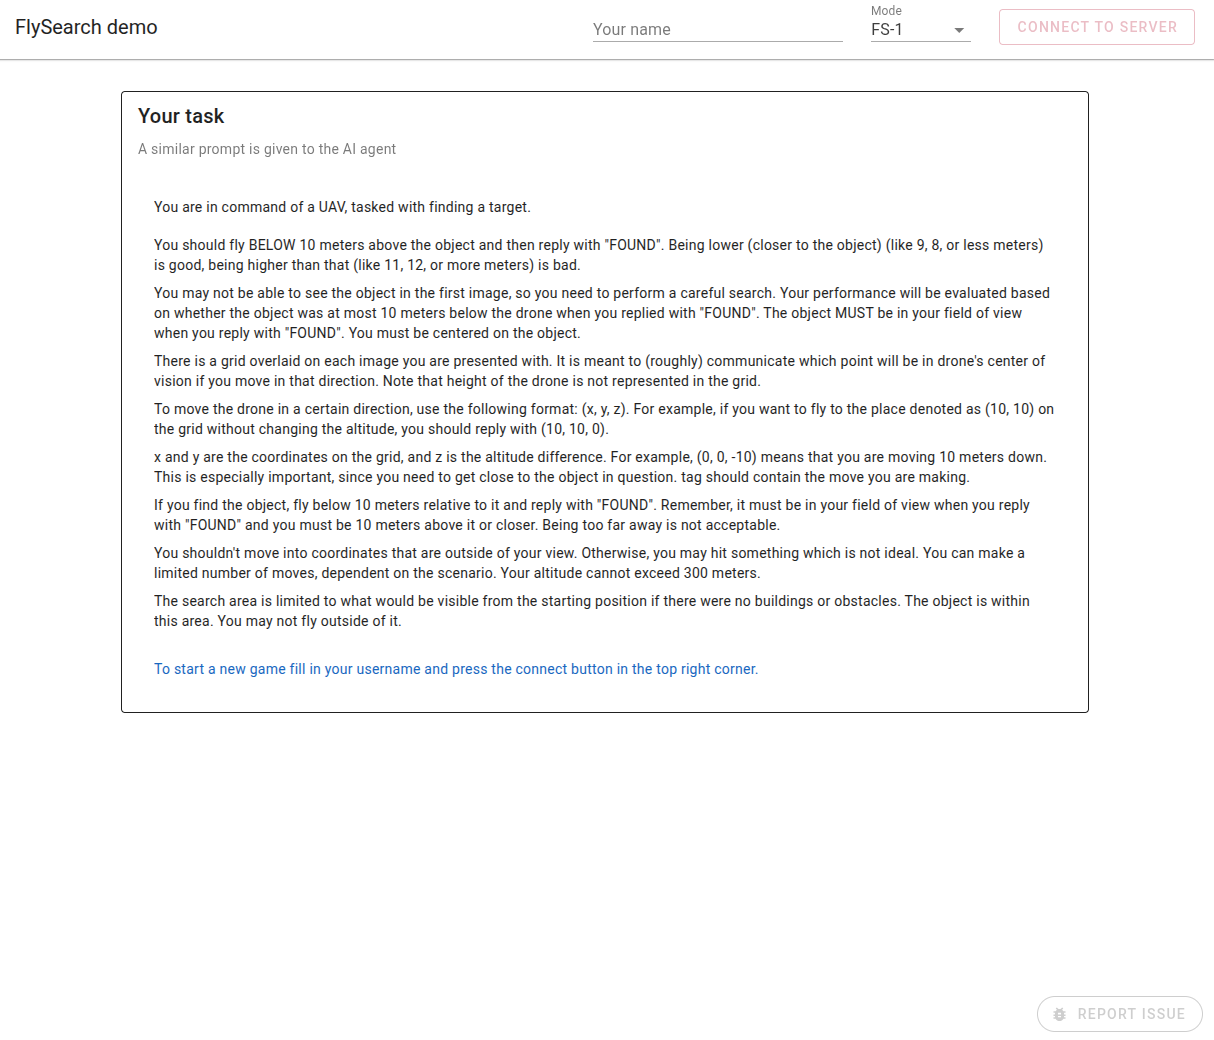
\includegraphics[width=.95\linewidth]{figs/human/start.png}}
    \caption{\textbf{Human study -- start screen}: Screenshot of the \ours{} human interface welcome screen, containing instructions derived from the benchmark prompt. The screen also contains a field for the participant identifier (nickname), a scenario generator switch (\challenge{}/\hardchallenge{}), connection button and bug report button.}
    \label{fig:web-start}
\end{figure*}

\begin{figure*}[ht]
    \centering
    \fbox{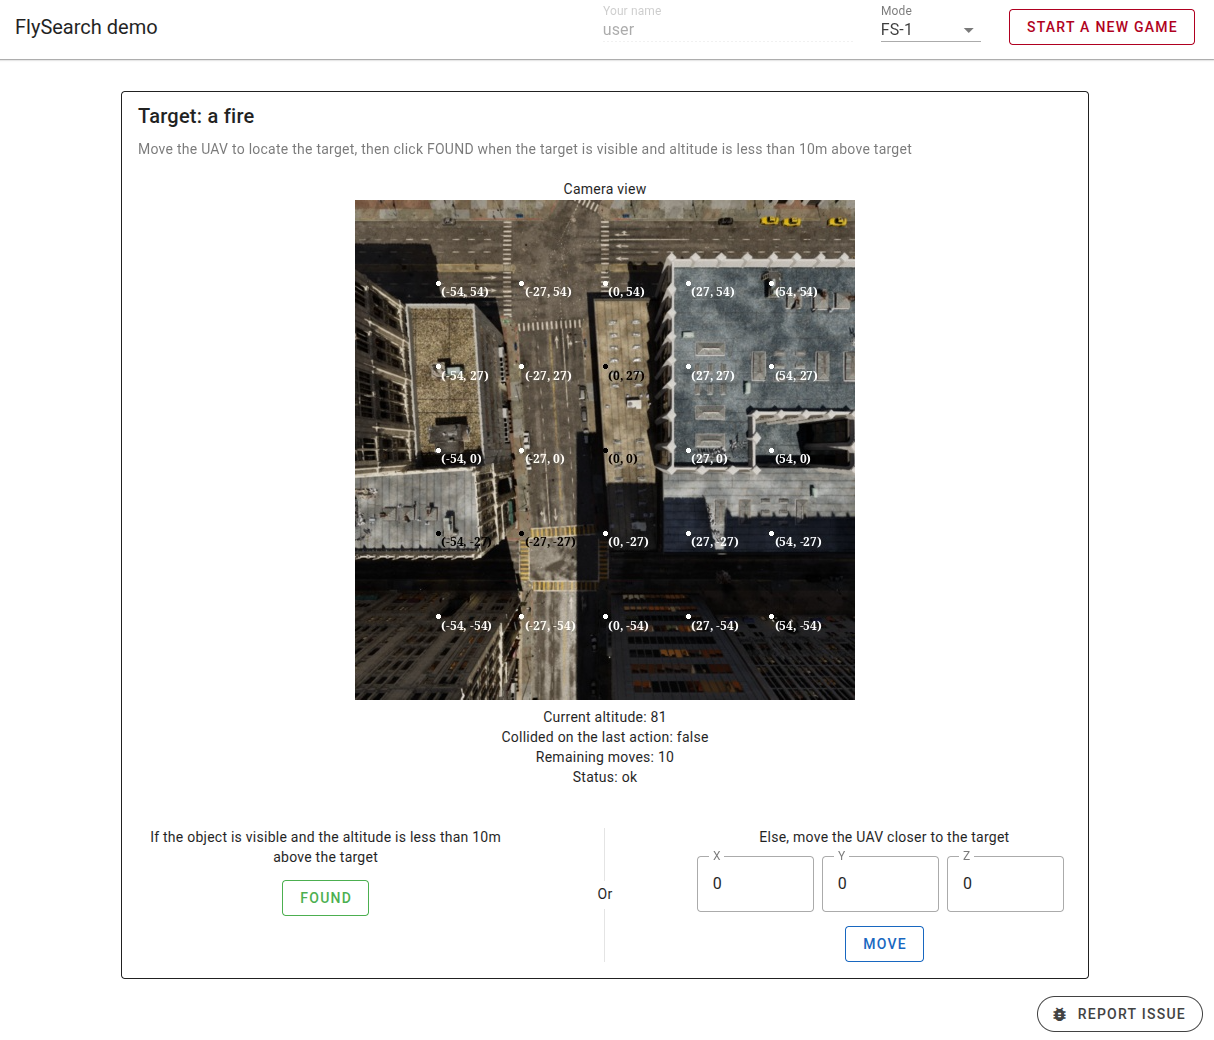
\includegraphics[width=.95\linewidth]{figs/human/fs1.png}}
    \caption{\textbf{Human study -- \challenge{} screen}: Screenshot of the \ours{} human interface \challenge{} screen. The page contains the target description, agent camera view, altitude, object and boundary collision information, and action controls. The image is overlaid with grid coordinates, exactly as the image provided to the evaluated VLM. All state and action elements are the same as those provided to the model, but for the formatting (a form instead of XML formatted text).}
    \label{fig:web-fs1}
\end{figure*}

\begin{figure*}[ht]
    \centering
    \fbox{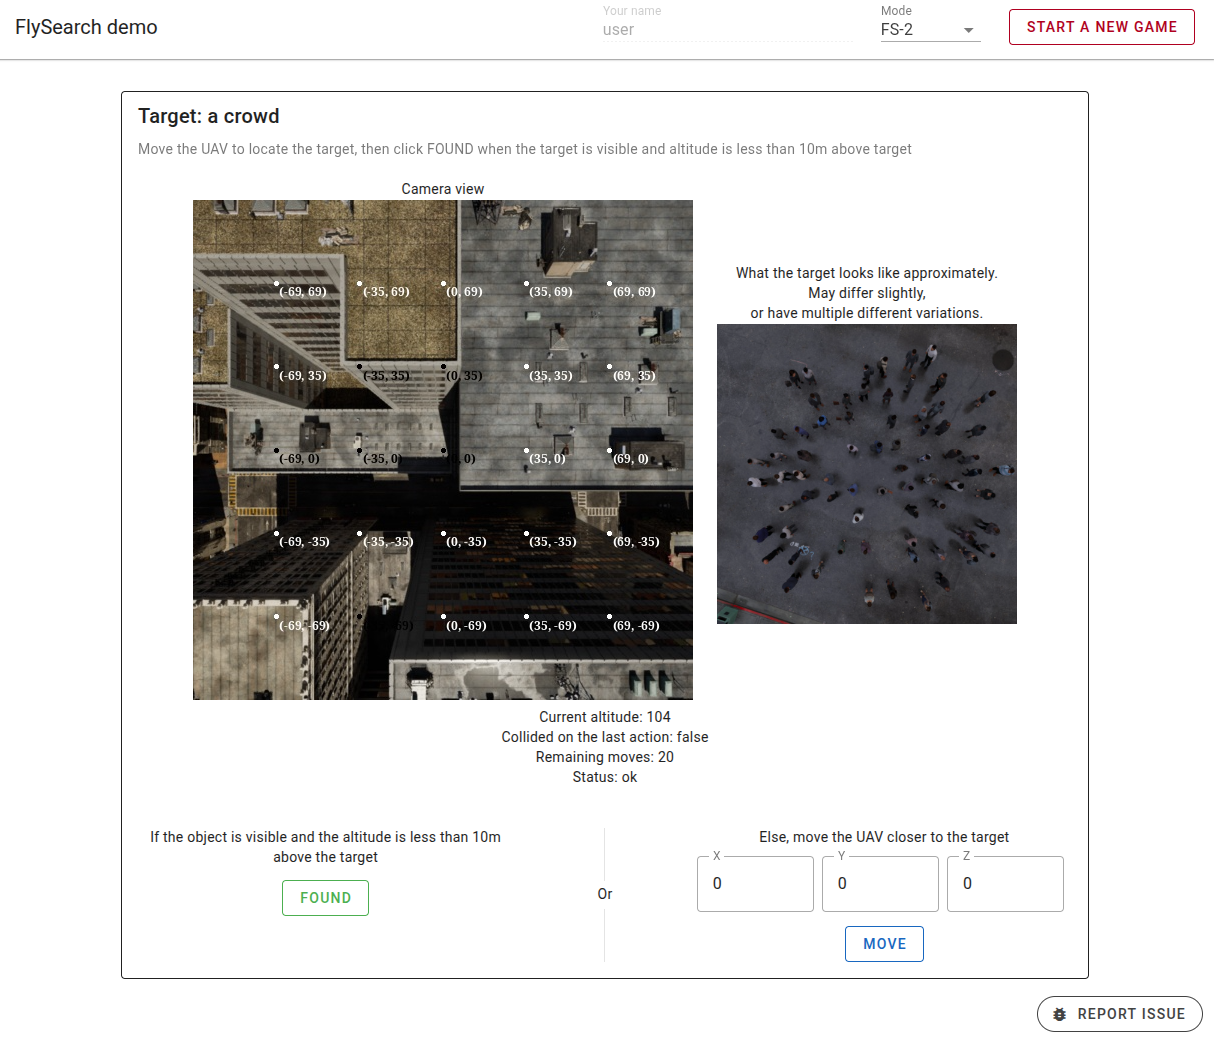
\includegraphics[width=.95\linewidth]{figs/human/fs2.png}}
    \caption{\textbf{Human study -- \hardchallenge{} screen}: Screenshot of the \ours{} human interface \hardchallenge{} screen. The page contains the same elements as for \challenge{} plus an additional visual description of the target (a neutral background and lightning picture, not an actual image of the searched object).}

    \label{fig:web-fs2}
\end{figure*}


\section{Fine-tuning details}
\label{app:finetune}

To provide a reasonable baseline score for fine-tuning VLMs for spatial reasoning we train the Qwen VL 2.5 7B~\cite{bai2025qwen2} model on the Forest environment and evaluate it on the City environment in both \challenge{} and \hardchallenge{}. The Qwen VL 2.5 7B model is selected as it is the best performing model in the \textit{small open-source model} category in our evaluation. Since the City and Forest environments share almost no graphical assets and are vastly different visually, training the model on Forest allows for a fair comparison with other models on the City environment. That is, the model cannot learn to visually recognize relevant objects and their placement in the evaluated scenario.

Using the Forest environment, we generate $6750$ unique exploration scenarios. In each scenario, we pre-record a flight trajectory from the starting point to the target. The trajectory is created by sampling $30$ evenly spaced steps over a straight line. To each flight step a random position offset in range of $[-10, 10]$ m, and capture camera views using our simulator. Finally, we augment the dataset by generating $10$ new trajectories from each captured episode, randomly dropping some of the flight steps. Resulting trajectories have between $1$ and $10$ steps, depending on the distance between start and target. Each trajectory is further cut at random step and formatted as a conversation to be completed by the VLM, resulting in $67500$ training samples.

Standard supervised fine-tuning does not provide sufficient improvement in results ($11.1\%$ on \challenge{} City, compared to $1.5\%$ of the base model). This is likely due to the fact, that each scenario can be solved in multiple ways, not just the ideal trajectory. Therefore, we apply GRPO fine-tuning~\cite{shao2024deepseekmath} in step-wise, offline manner. That is, using the pre-generated training dataset we train the model to predict one next action. We define the reward function for the step with the following pseudo-code:

\begin{lstlisting}[caption=Reward for GRPO fine-tuning (pseudo-code).,label={lst:rewardgrpo}]
def reward(model_output):
    if model_output is not parsable:
        return 0
        
    reasoning, action = parse(model_output)
    
    reasoning_reward = min(1, len(reasoning) / 100)

    if action == 'FOUND':
        if target_located:
            return 1 + reasoning_reward
        else:
            return 0 + reasoning_reward

    action_reward = (current_distance - next_distance) / current_distance
    action_reward = max(min(action_reward, 1), 0) # clip between 0 and 1

    if target_located:
        # action should be FOUND, decrease reward for further moves
        mod = max(0., (altitude - targed_height compare)) / 10
        action_reward = (mod ** .5) * action_reward

    return reasoning_reward + action_reward
\end{lstlisting}

Therefore, the model is incentivized to both provide at least $100$ tokens of reasoning output and to move closer to the target in each step. When the model can respond with \texttt{FOUND} action the reward for further moves towards the target is decreased. Finally, if the agent responds with \texttt{FOUND} it receives a binary reward based on the success.

We perform the GRPO fine-tuning using the Swift library~\cite{zhao2024swiftascalablelightweightinfrastructure}, and use LoRA~\cite{hu2022lora} to speed up the training. Moreover, we freeze the vision encoder part of the model to prevent overfitting on visual features. Bellow are the full parameters of the training:
\begin{lstlisting}[caption=GRPO fine-tuning command.,label={lst:paramsgrpo}]
NPROC_PER_NODE=2 CUDA_VISIBLE_DEVICES=0,1,2,3 swift rlhf \
  --rlhf_type grpo \
  --model Qwen/Qwen2.5-VL-7B-Instruct \
  --train_type lora \
  --dataset $DATA_PATH \
  --num_train_epochs 1 \
  --per_device_train_batch_size 8 \
  --per_device_eval_batch_size 8 \
  --learning_rate 1e-5 \
  --gradient_accumulation_steps 1 \
  --eval_steps 100 \
  --save_steps 100 \
  --save_total_limit 2 \
  --logging_steps 5 \
  --dataloader_num_workers 4 \
  --attn_impl flash_attn \
  --use-hf \
  --torch_dtype bfloat16 \
  --deepspeed zero2 \
  --target_modules all-linear lm_head \
  --lora_alpha 32 \
  --lora_rank 8 \
  --external_plugins rewardplugin.py \
  --reward_funcs fly_search \
  --max_completion_length 1024 \
  --warmup_ratio 0.05 \
  --num_generations 16 \
  --dataset_num_proc 4 \
  --temperature 0.9 \
  --log_completions true \
  --use_vllm true \
  --vllm_gpu_memory_utilization 0.9 \
  --vllm_limit_mm_per_prompt '{"image": 10}' \
  --num_infer_workers 2 \
  --async_generate true \
  --seed 42 \
  --split_dataset_ratio 0
\end{lstlisting}
The entire process takes several hours using 4 NVIDIA H100 GPUs. After fine-tuning the model is evaluated with standard \challenge{} City and \hardchallenge{} settings, achieving $27.0\%$ and $0.0\%$ accordingly. Moreover, it achieves $57.0\%$ accuracy on the Forest environment it was trained upon.

\section{Success criterion implementation}
\label{sec:success_impl}

\begin{figure}[h]
\begin{center}
    \begin{tikzpicture}[scale=2]

    \draw[thick] (-2,-2) -- (0, 0);
    \draw[thick] (0, 0) -- (2, -2);

    \draw[black,thick,dashed] (0, 0) -- (0, -2);

    \tkzDefPoints{-2/-2/A,0/0/B,2/-2/C,0/-2/D};
    \tkzMarkRightAngle[size = 0.25](A,B,C);
    \tkzMarkRightAngle[size = 0.25](B,D,C);


    \tkzMarkAngle[size = 0.75, arc=l,mkcolor,mkpos=.33](B,C,D);
    \tkzLabelAngle[dist=0.5](B,C,D){\(45\degree\)};

    \tkzMarkAngle[size = 0.75, arc=l,mkcolor,mkpos=.33](D,A,B);
    \tkzLabelAngle[dist=0.5](D,A,B){\(45\degree\)};

    \tkzLabelPoint[above, black](B){Agent's location};

    \tkzDefPoints{0/-1/H,0.75/-2/L, -0.75/-2/L2};
    \tkzLabelPoint[right,  black](H){\(h\)};
    \tkzLabelPoint[above,  black](L){\(h\)};
    \tkzLabelPoint[above,  black](L2){\(h\)};

    \draw[black, thick, dashed] (-2, -2) -- (2, -2);

    \end{tikzpicture}
\end{center}
    \caption{\textbf{Success criterion illustration:} The searched object's center must be inside of the camera's cone of view. We assume the camera's field of view is $90\degree$.}
    \label{fig:metricdraw}
\end{figure}

For a trajectory to be considered successful, at the end of it the agent must be located less than 10 meters above the object's highest point. Furthermore, the object must be seen from the agent's location.

To check whether the agent can see the object, we calculate agent's cone of view and check whether object's center is inside of the cone of view. This calculation is straightforward, because camera's field of view is \(90\degree\). It easily follows that agent at altitude \(h\) sees an area of \(2h \times 2h\) meters. We provide a drawing to illustrate that fact in Fig.~\ref{fig:metricdraw}.

In some cases, this implementation may cause misclassifications as a failure, due to the agent ,,seeing'' an object in a human sense (e.g. a significant part of it's edges), but not having object's center in its cone of view. To avoid this issue, we specify in the prompt that agent should be \textit{centered} on the object.

\section{Prompt templates}

In this section we present the prompt templates for all benchmark tasks.

\label{sec:prompt}

\subsection{Prompt template for \challenge{} and \anomalychallenge{}}

\input{figs/fs1prompt}

\subsection{Prompt template for \hardchallenge{}}

\input{figs/fs2prompt}

Furthermore, along with the textual description of the searched object we pass the image, showcasing how it should look like from above, with a following annotation: 

\begin{lstlisting}[caption=Annotation of searched object's image in \hardchallenge{}.,label={lst:anno}]
The object you're looking for is similar to this. This is NOT the drone's current view.
\end{lstlisting}


\section{Additional Experiments}

In this section we present additional experimental results, evaluating design choices of our benchmark.

\label{app:additional_exps}
\begin{table*}[ht]
\centering
\footnotesize
\caption{Performance of Gemini 2.0 Flash and Pixtral-Large on ablations.}
\label{tab:ablations2}
\begin{tabular}{llcccc}
\toprule
& \multirow{2}{*}{\textbf{Setting}} & \multicolumn{2}{c}{\textbf{City}} & \multicolumn{2}{c}{\textbf{Forest}} \\
\cmidrule(lr){3-4} \cmidrule(lr){5-6}
&& \textbf{Gemini} & \textbf{Pixtral} & \textbf{Gemini} & \textbf{Pixtral} \\
\midrule
\multirow{3}{*}{\challenge{}} & \textbf{Baseline} & $\mathbf{41.5\%}$ & $\mathbf{21.5\%}$ & $\mathbf{42.5\%}$ & $\mathbf{38.0\%}$ \\
& Compass actions & $17.5\%$ & $21.0\%$ & $17.5\%$ & $22.0\%$ \\
& No grid overlay & $17.0\%$ & $15.5\%$ & $31.5\%$ & $20.0\%$ \\
\midrule
\multirow{2}{*}{FS-Anomaly} & \textbf{Baseline} & $25.0\%$ & $4.0\%$ & $46.0\%$ & $26.0\%$ \\
& Anomaly with ID & $\mathbf{34.0\%}$ & $\mathbf{7.0\%}$ & $\mathbf{59.0\%}$ & $\mathbf{34.0\%}$ \\
\bottomrule \\
\end{tabular}
\end{table*}

\begin{table}[th]
    \centering
    \begin{footnotesize}
    \caption{\textbf{\anomalychallenge{} results:} Success rates ($\pm$ standard errors) of the evaluated models.}
\label{tab:main_results_anomaly_app}
    \begin{tabular}{lccc}
\toprule
\multirow{2}{*}{Model}& \multicolumn{3}{c}{\anomalychallenge{}} \\
\cmidrule(lr){2-4}
 & Overall (\%) & Forest (\%) & City (\%)\\
\midrule
GPT-4o & $ 27.0 \pm 3.1 $ & $ 39.0 \pm 4.9 $ & $ 15.0 \pm 3.6 $ \\
Claude 3.5 Sonnet & $ 27.5 \pm 3.2 $ & $ 37.0 \pm 4.9 $ & $ 18.0 \pm 3.9 $ \\
Gemini 2.0 flash & $ \mathbf{35.5 \pm 3.4} $ & $ \mathbf{46.0 \pm 5.0} $ & $ \mathbf{25.0 \pm 4.4} $ \\
\midrule
Phi 3.5 vision & $ 0.0 \pm 0.0 $ & $ 0.0 \pm 0.0 $ & $ 0.0 \pm 0.0 $ \\
InternVL-2.5 8B MPO & $ 3.5 \pm 1.3 $ & $ 6.0 \pm 2.4 $ & $ 1.0 \pm 1.0 $ \\
Llava-Interleave-7b & $ 0.0 \pm 0.0 $ & $ 0.0 \pm 0.0 $ & $ 0.0 \pm 0.0 $ \\
Qwen2.5-VL 7B & $ 2.8 \pm 1.2 $ & $ 3.7 \pm 2.1 $ & $ 2.0 \pm 1.4 $ \\
\midrule
Qwen2-VL-72B & $ 7.5 \pm 1.9 $ & $ 10.0 \pm 3.0 $ & $ 5.0 \pm 2.2 $ \\
Llava-Onevision 72b & $ 8.5 \pm 2.0 $ & $ 11.0 \pm 3.1 $ & $ 6.0 \pm 2.4 $ \\
Pixtral-Large & $ 15.0 \pm 2.5 $ & $ 26.0 \pm 4.4 $ & $ 4.0 \pm 2.0 $ \\
\bottomrule
\end{tabular}
\end{footnotesize}
\end{table}
\begin{figure*}[t]
\begin{small}
\centering
\begin{subfigure}{0.47\linewidth}
    \begin{tikzpicture}
    \centering
    \begin{axis}[
        title={Forest},
        height=5cm,
        width=.9\linewidth,
        xlabel={Starting altitude (meters)},
        ylabel={Succes},
        yticklabel={\pgfmathprintnumber\tick\%},
        xtick={30,40,50,60, 70, 80, 90},
        xticklabels={$[30{,}40)$, $[40{,}50)$, $[50{,}60)$, $[60{,}70)$, $[70{,}80)$, $[80{,}90)$,$[90{,}100)$},
        xticklabel style={rotate=45,anchor=east,yshift=-.2cm},
        xmin=30, xmax=90,
        ymin=0, ymax=100,
        ytick={0,20,40,60,80,100},
        %legend pos=north east,
        ymajorgrids=true,
        xmajorgrids=true,
        grid style=dashed,
        legend to name=altitude-anchor,
        legend columns=3,
        legend style={nodes={scale=0.8, transform shape}},
        legend cell align={left},
        every axis plot/.append style={thick}
    ]

\addplot[color=color0, mark=square]
coordinates {
(30.0, 73.9)
(40.0, 64.5)
(50.0, 48.6)
(60.0, 56.0)
(70.0, 28.1)
(80.0, 30.4)
(90.0, 20.7)
};
\addlegendentry{GPT-4o}
\addplot[color=color1, mark=square]
coordinates {
(30.0, 73.9)
(40.0, 61.3)
(50.0, 59.5)
(60.0, 48.0)
(70.0, 31.2)
(80.0, 52.2)
(90.0, 41.4)
};
\addlegendentry{Claude 3.5 Sonnet}
\addplot[color=color2, mark=square]
coordinates {
(30.0, 56.5)
(40.0, 58.1)
(50.0, 46.0)
(60.0, 52.0)
(70.0, 34.4)
(80.0, 34.8)
(90.0, 17.2)
};
\addlegendentry{Gemini 2.0 Flash}
% \addplot[color=color3, mark=square]
% coordinates {
% (30.0, 0.0)
% (40.0, 0.0)
% (50.0, 0.0)
% (60.0, 0.0)
% (70.0, 0.0)
% (80.0, 0.0)
% (90.0, 0.0)
% };
% \addlegendentry{Phi 3.5 vision}
% \addplot[color=color4, mark=square]
% coordinates {
% (30.0, 4.3)
% (40.0, 3.2)
% (50.0, 2.7)
% (60.0, 8.0)
% (70.0, 0.0)
% (80.0, 0.0)
% (90.0, 6.9)
% };
% \addlegendentry{InternVL-2.5 8B MPO}
% \addplot[color=color5, mark=square]
% coordinates {
% (30.0, 0.0)
% (40.0, 3.2)
% (50.0, 0.0)
% (60.0, 4.0)
% (70.0, 0.0)
% (80.0, 0.0)
% (90.0, 3.5)
% };
% \addlegendentry{Llava-Interleave 7b}
\addplot[color=color6, mark=square]
coordinates {
(30.0, 21.7)
(40.0, 16.1)
(50.0, 13.5)
(60.0, 20.0)
(70.0, 12.5)
(80.0, 17.4)
(90.0, 13.8)
};
\addlegendentry{Qwen2-VL 72B}
\addplot[color=color7, mark=square]
coordinates {
(30.0, 39.1)
(40.0, 19.4)
(50.0, 16.2)
(60.0, 20.0)
(70.0, 3.1)
(80.0, 26.1)
(90.0, 10.3)
};
\addlegendentry{Llava-Onevision 72b}
\addplot[color=color8, mark=square]
coordinates {
(30.0, 43.5)
(40.0, 48.4)
(50.0, 46.0)
(60.0, 44.0)
(70.0, 31.2)
(80.0, 26.1)
(90.0, 24.1)
};
\addlegendentry{Pixtral-Large 124B}

\end{axis}

\end{tikzpicture}
\end{subfigure}
\begin{subfigure}{0.47\linewidth}
\centering
    \begin{tikzpicture}
     \begin{axis}[
        title={City},
        height=5cm,
        width=.9\linewidth,
        xlabel={Starting altitude (meters)},
        ylabel={Succes},
        yticklabel={\pgfmathprintnumber\tick\%},
        xtick={30,40,50,60, 70, 80, 90},
        xticklabel={},
        xticklabels={$[30{,}40)$, $[40{,}50)$, $[50{,}60)$, $[60{,}70)$, $[70{,}80)$, $[80{,}90)$,$[90{,}100)$},
        xticklabel style={rotate=45,anchor=east,yshift=-.2cm},
        xmin=30, xmax=90,
        ymin=0, ymax=100,
        ytick={0,20,40,60,80,100},
        %legend pos=north east,
        ymajorgrids=true,
        xmajorgrids=true,
        grid style=dashed,
        every axis plot/.append style={thick}
    ]

\addplot[color=color0, mark=square]
coordinates {
(30.0, 71.4)
(40.0, 45.8)
(50.0, 35.3)
(60.0, 25.9)
(70.0, 13.8)
(80.0, 3.6)
(90.0, 12.5)
};
\addplot[color=color1, mark=square]
coordinates {
(30.0, 61.9)
(40.0, 45.8)
(50.0, 23.5)
(60.0, 25.9)
(70.0, 13.8)
(80.0, 14.3)
(90.0, 6.2)
};
\addplot[color=color2, mark=square]
coordinates {
(30.0, 78.6)
(40.0, 50.0)
(50.0, 38.2)
(60.0, 25.9)
(70.0, 34.5)
(80.0, 21.4)
(90.0, 12.5)
};
% \addplot[color=color3, mark=square]
% coordinates {
% (30.0, 0.0)
% (40.0, 0.0)
% (50.0, 0.0)
% (60.0, 0.0)
% (70.0, 0.0)
% (80.0, 0.0)
% (90.0, 0.0)
% };
% \addplot[color=color4, mark=square]
% coordinates {
% (30.0, 4.8)
% (40.0, 4.2)
% (50.0, 0.0)
% (60.0, 0.0)
% (70.0, 0.0)
% (80.0, 0.0)
% (90.0, 0.0)
% };
% \addplot[color=color5, mark=square]
% coordinates {
% (30.0, 4.8)
% (40.0, 4.2)
% (50.0, 0.0)
% (60.0, 0.0)
% (70.0, 0.0)
% (80.0, 0.0)
% (90.0, 0.0)
% };
\addplot[color=color6, mark=square]
coordinates {
(30.0, 38.1)
(40.0, 29.2)
(50.0, 11.8)
(60.0, 11.1)
(70.0, 10.3)
(80.0, 3.6)
(90.0, 12.5)
};
\addplot[color=color7, mark=square]
coordinates {
(30.0, 26.2)
(40.0, 8.3)
(50.0, 17.6)
(60.0, 3.7)
(70.0, 3.5)
(80.0, 3.6)
(90.0, 6.2)
};
\addplot[color=color8, mark=square]
coordinates {
(30.0, 47.6)
(40.0, 25.0)
(50.0, 14.7)
(60.0, 18.5)
(70.0, 17.2)
(80.0, 3.6)
(90.0, 6.2)
};
  
\end{axis}
\end{tikzpicture}

\end{subfigure}
\end{small}
\centering
\begin{tikzpicture}
\node[anchor=north] at (current axis.below south) {\ref{altitude-anchor}};
\end{tikzpicture}

\caption{\textbf{Success rate per starting altitude interval:} In this figure, we plot the success rates of the models as a function of the initial altitude interval for both the Forest and the City environments in the \challenge{} challenge. The performance drop that comes with increasing altitude is more pronounced for the City environment.}
    \label{fig:by_altitude}
\end{figure*}


\paragraph{Impact of the action space.}
We test how changing the action format affects performance by replacing the default Cartesian $(x, y, z)$ movements with compass-style commands that specify a direction (north, south, east, west, up, down) and distance. This type of action space is common in previous works. As shown in Table~\ref{tab:ablations2}, this change significantly degrades performance for both Gemini 2.0 Flash and Pixtral-Large. Gemini’s accuracy drops from 42.5\% to 17.5\% in Forest and from 41.5\% to 17.5\% in City. Pixtral falls from 38\% to 22\% in Forest, with little change in City (21.5\% to 21\%).
These results highlight the importance of a flexible, continuous action space. Compass-style movement restricts fine-grained control and appears to limit the models’ ability to effectively search.

\paragraph{Impact of the grid overlay.}
To assess the importance of the grid overlay on each glimpse, we run an ablation where glimpses are shown without the grid.
As shown in Table~\ref{tab:ablations2}, removing the grid leads to a notable drop in performance for both Gemini 2.0 Flash and Pixtral-Large. Gemini’s success rate falls from 42.5\% to 31.5\% in Forest, and more dramatically in City—from 41.5\% to 17\%. Pixtral shows a similar trend, dropping from 38\% to 20\% in Forest and from 21.5\% to 15.5\% in City.
These results suggest that the grid plays a key role in helping models maintain spatial awareness, especially in more complex environments. Without it, both localization and goal-oriented planning appear to suffer. This result is consistent with previous works on vision-language coordination~\cite{lei2024scaffolding}.

\paragraph{Impact of hidden vs explicit anomaly categories.}
In the FS-Anomaly setting, the model must identify an object that doesn’t belong in the surrounding environment. In the base version, the anomaly category is implicit, requiring the model to infer what is out of place. In this ablation, we explicitly tell the model what object to look for.

As shown in Table~\ref{tab:ablations2}, providing the anomaly identity significantly improves performance. Gemini's accuracy increases from 46\% to 59\% in Forest and from 25\% to 34\% in City. Pixtral also improves, from 26\% to 34\% in Forest and from 4\% to 7\% in City.

This result suggests that models often struggle with anomaly detection due to semantic ambiguity rather than visual perception. Explicitly stating the anomaly class helps disambiguate the task and leads to more focused and successful exploration.

\textbf{\anomalychallenge{} full results.}
We provide full results of the \anomalychallenge{} benchmark with distinction between Forest and City environment performance in \cref{tab:main_results_anomaly_app}.

\textbf{Impact of the starting height.}
Finally, we verify how the results vary depending on the starting height.
As seen in \cref{fig:by_altitude}, the success rate decreases as the starting altitude (and therefore distance to the target) increases. This is particularly significant in the City environment, where the success rate for the best models drops by half, likely due to the high number of distracting objects. In contrast, in the generally easier Forest environment, this decline is less pronounced and occurs mainly in the upper half of the altitude range.

\section{Sim2real gap}
The main design goal of FlySearch is the evaluation of VLM exploration and 3D spatial reasoning capabilities, with UAV object navigation serving as a realistic assessment task. However, we acknowledge the fact that FlySearch can serve as a platform for testing methods designed specifically for UAV control, including non-VLM solutions. Therefore, in this section, we discuss in depth the differences between FlySearch and real-life UAV control, underlining issues that were simplified or omitted in order for the problem to be addressable with existing foundational VLMs.

\paragraph{Environment.} FlySearch uses Unreal Engine 5 to provide near-photorealistic simulation of highly complex environments, with both procedurally generated and handcrafted content, using a vast set of high-resolution assets and generation rules. This setup allows for world simulation on par with the latest video games. However, the real world presents far greater complexity and unpredictability than any video game. This might lead to discrepancies between the behavior of VLM in simulated and real-world environments.
\paragraph{World dynamics.} The real world contains a vast number of dynamic elements (moving cars, walking people, flying birds, etc.) that cannot be fully simulated even with modern video game engines. Moreover, FlySearch omits some of the flight-related dynamics, such as sudden gusts of wind or abrupt weather changes, that were deemed too complex for current foundational VLMs.
\paragraph{Sensor simulation.} Our benchmark limits sensor inputs to a downward-facing camera and altitude reading with 1 m accuracy. The camera sensor is simulated using real-time ray-tracing capabilities of the engine, accounting for camera auto-exposure, depth of view, light direction (time of the day), fixed light cloud cover, and atmospheric haze. This enables an overall realistic simulation of a modern digital camera, but simplifies the weather element and omits any data loss or low-light condition emulation. Furthermore, real-life platforms may feature multiple cameras, LIDAR/RADAR, GPS units, IMU, and other sensor modalities that are not simulated in FlySearch.
\paragraph{Target objects.} The searched object is stationary (may be animated but remains in the same location), unique for the scenario (visually similar but semantically different objects may exist on the map), and visible from the top. In real-world situations, the object can move freely in the environment, including moving inside buildings, and the description of the object provided to the agent can match multiple objects. It may require more complex search strategies and the cooperation of multiple agents.
\paragraph{UAV control.} FlySearch uses high-level relative movement actions with 1 m resolution. This can be implemented in real-life UAVs using existing autopilot software such as PX4 Autopilot or DroneKit, which can accommodate wind changes and drift. However, a more direct control of the platform could speed up the exploration process in practice and make it less dependent on GPS or inertial navigation systems. At the same time, this makes the task more complex for both VLM models and human evaluators.
\paragraph{Other simplifications.} The benchmark limits agent interaction with the world to up to 20 steps due to the model context length limitations of most open-source VLMs. In real-life problems, the location of an object in a large environment may require significantly more observations. In addition, real-world UAVs are subject to hardware and software failures, none of which are simulated in FlySearch.
In future work, when VLMs can solve our toughest challenge set, we plan to address some of the above limitations, making our benchmark more realistic.


\section{Example trajectories}

\label{app:trajectories}

The sample trajectories of different VLMs on \challenge{} and \hardchallenge{} scenarios are provided in a separate file in the supplementary material, as well as at: \url{https://github.com/gmum/FlySearch/blob/main/docs/example-trajectories.pdf}


\input{appendix/checklist}
